% ══════════════════════════════════════════════════════════════
% LaTeX 论文片段：跨学科知识图谱构建与 Benchmark GT 数据集
% ══════════════════════════════════════════════════════════════

% ── 所需宏包 ──
% \usepackage{amsmath, amssymb, booktabs, algorithm, algorithmic, graphicx, multirow}

% ══════════════════════════════════════════════════════════════
% Section: 形式化定义
% ══════════════════════════════════════════════════════════════

\subsection{Cross-Disciplinary Knowledge Graph}

\begin{definition}[Cross-Disciplinary Knowledge Graph]
For a paper $p$, we define its knowledge graph as a directed attributed graph $G_p = (V, E, \phi, \psi)$, where:
\begin{itemize}
    \item $V = \{v_1, \ldots, v_n\}$ is the set of concept nodes. Each node $v_i$ carries attributes $(\textit{term}_i, \textit{normalized}_i, \textit{discipline}_i, \textit{evidence}_i, \textit{confidence}_i \in [0,1])$.
    \item $E \subseteq V \times V \times \mathcal{R}$ is the set of typed directed edges, where $\mathcal{R}$ is a predefined relation type vocabulary containing 16 types (see Table~\ref{tab:relation_types}).
    \item $\phi: V \to \mathcal{D}$ maps each node to its discipline from the MSC taxonomy $\mathcal{D}$.
    \item $\psi: E \to [0,1]$ assigns confidence scores to each edge based on extraction certainty.
\end{itemize}
\end{definition}

\begin{definition}[Hypothesis Path]
A hypothesis path at level $\ell \in \{L1, L2, L3\}$ is an ordered sequence of reasoning steps $\mathcal{P}^{(\ell)} = [s_1, s_2, s_3]$, where each step $s_k = (\textit{head}_k, \textit{relation}_k, \textit{tail}_k, \textit{claim}_k)$ represents a knowledge assertion linking two concepts across potentially different disciplines. The three levels capture macro-level interdisciplinary bridging (L1), meso-level mechanism reasoning (L2), and micro-level precise inference chains (L3).
\end{definition}


% ══════════════════════════════════════════════════════════════
% Section: 算法
% ══════════════════════════════════════════════════════════════

\subsection{Knowledge Graph Construction Algorithm}

\begin{algorithm}[t]
\caption{Multi-Stage Knowledge Graph Construction}
\label{alg:kg_construction}
\begin{algorithmic}[1]
\REQUIRE Paper $p = (\textit{title}, \textit{abstract}, \textit{introduction}, \textit{disciplines})$
\ENSURE Knowledge graph $G_p = (V, E)$ with metrics $\mathbf{m}$
\STATE \textbf{Stage 1a:} $V_{\text{init}} \leftarrow \textsc{ConceptExtraction}(p)$ \COMMENT{LLM-based}
\STATE \textbf{Stage 1b:} $V_{\text{supp}} \leftarrow \textsc{SupplementExtraction}(p, V_{\text{init}})$ \COMMENT{Gap-filling}
\STATE $V \leftarrow \textsc{Deduplicate}(V_{\text{init}} \cup V_{\text{supp}})$
\STATE $V \leftarrow \textsc{GroundAndFilter}(V, \mathcal{T}_{\text{MSC}})$ \COMMENT{Taxonomy grounding}
\STATE \textbf{Stage 2a:} $E_{\text{struct}} \leftarrow \textsc{RelationExtraction}(p, V)$ \COMMENT{With evidence}
\STATE \textbf{Stage 2b:} $Q \leftarrow \textsc{QueryGeneration}(V, E_{\text{struct}})$ \COMMENT{3-level queries}
\STATE \textbf{Stage 3:} \COMMENT{Parallel L1/L2/L3 hypothesis generation}
\FORALL{$\ell \in \{L1, L2, L3\}$ \textbf{in parallel}}
    \STATE $\mathcal{P}^{(\ell)} \leftarrow \textsc{HypothesisGeneration}(V, E_{\text{struct}}, Q, \ell)$
    \STATE $\mathcal{P}^{(\ell)} \leftarrow \textsc{EntityAlignment}(\mathcal{P}^{(\ell)}, V)$ \COMMENT{Fuzzy match $\geq 0.70$}
\ENDFOR
\STATE $E_{\text{hyp}} \leftarrow \bigcup_\ell \textsc{PathsToEdges}(\mathcal{P}^{(\ell)})$
\STATE $G_p \leftarrow (V, E_{\text{struct}} \cup E_{\text{hyp}})$
\STATE $\mathbf{m} \leftarrow \textsc{ComputeMetrics}(G_p, E_{\text{struct}}, E_{\text{hyp}})$ \COMMENT{24 metrics}
\RETURN $G_p, \mathbf{m}$
\end{algorithmic}
\end{algorithm}


\begin{algorithm}[t]
\caption{Evidence-Grounded Benchmark GT Construction}
\label{alg:gt_construction}
\begin{algorithmic}[1]
\REQUIRE Extraction result $r$ with parsed concepts and text content
\ENSURE Benchmark entry $b = (\textit{input}, \textit{ground\_truth}, \textit{stats})$
\STATE \textbf{Stage 1:} $T \leftarrow \textsc{ConstrainedTermExtraction}(r)$
\STATE $T \leftarrow \textsc{DictionaryGrounding}(T, \mathcal{T}_{\text{MSC}})$
\STATE \textbf{Stage 2:} $\textit{sents} \leftarrow \textsc{SentenceSplit}(r.\textit{abstract} \| r.\textit{introduction})$
\FORALL{sentence $s \in \textit{sents}$}
    \STATE $\textit{co\_terms} \leftarrow \{t \in T : t \text{ appears in } s\}$
    \FORALL{$(t_i, t_j) \in \binom{\textit{co\_terms}}{2}$}
        \STATE $R \leftarrow R \cup \{(t_i, t_j, \textsc{ClassifyRelation}(s, t_i, t_j))\}$
    \ENDFOR
\ENDFOR
\STATE \textbf{Stage 3:} $\mathcal{G} \leftarrow \textsc{BuildGraph}(T, R)$ \COMMENT{NetworkX DiGraph}
\STATE $\textit{Paths} \leftarrow \textsc{CrossDisciplinaryTraversal}(\mathcal{G}, \text{max\_len}=k)$
\STATE $\textit{stats} \leftarrow \textsc{ComputeStats}(T, R, \textit{Paths})$
\RETURN $b$
\end{algorithmic}
\end{algorithm}


% ══════════════════════════════════════════════════════════════
% Section: 指标公式
% ══════════════════════════════════════════════════════════════

\subsection{Quality Metrics}

\paragraph{Path Consistency.}
Measures the proportion of hypothesis edges that align with evidence-grounded structural edges:
\begin{equation}
    \text{PathConsistency} = \frac{|\{e \in E_{\text{hyp}} : e \in E_{\text{struct}}\}|}{|E_{\text{hyp}}|}
\end{equation}

\paragraph{Concept Coverage.}
Fraction of structural concept nodes covered by at least one hypothesis path:
\begin{equation}
    \text{Coverage} = \frac{|\{v \in V_{\text{struct}} : \exists\, \mathcal{P}^{(\ell)} \text{ s.t. } v \in \mathcal{P}^{(\ell)}\}|}{|V_{\text{struct}}|}
\end{equation}

\paragraph{Bridging Score.}
Fraction of edges connecting nodes from \emph{different} disciplines, restricted to edges with valid discipline annotations:
\begin{equation}
    \text{Bridging} = \frac{|\{(u,v) \in E : \phi(u) \neq \phi(v)\}|}{|\{(u,v) \in E : \phi(u), \phi(v) \notin \mathcal{D}_{\text{invalid}}\}|}
\end{equation}

\paragraph{Rao-Stirling Diversity.}
Quantifies the disciplinary diversity of concepts used in hypothesis paths:
\begin{equation}
    \Delta_{\text{RS}} = \sum_{i \neq j} d_{ij} \cdot p_i \cdot p_j
\end{equation}
where $d_{ij}$ is the taxonomic distance between disciplines $i$ and $j$, and $p_i$ is the proportion of hypothesis steps involving discipline $i$.

\paragraph{Chain Coherence.}
Average semantic coherence across all reasoning chains, computed using embedding similarity between consecutive steps:
\begin{equation}
    \text{Coherence} = \frac{1}{|\mathcal{P}|} \sum_{\mathcal{P}^{(\ell)}} \frac{1}{|\mathcal{P}^{(\ell)}|-1} \sum_{k=1}^{|\mathcal{P}^{(\ell)}|-1} \cos(\mathbf{e}_{s_k}, \mathbf{e}_{s_{k+1}})
\end{equation}


% ══════════════════════════════════════════════════════════════
% Section: 实验结果表格
% ══════════════════════════════════════════════════════════════

\subsection{Experimental Results}


\begin{table}[t]
\centering
\caption{Knowledge Graph Construction Statistics (94 papers).}
\label{tab:kg_stats}
\begin{tabular}{lcccc}
\toprule
\textbf{Statistic} & \textbf{Mean} & \textbf{Std} & \textbf{Min} & \textbf{Max} \\
\midrule
Nodes per paper  & 28.8 & 6.0 & 20 & 54 \\
Edges per paper  & 27.1 & 2.9 & 19 & 34 \\
L1 paths/paper   & 2.5 & 0.5 & 1 & 3 \\
L2 paths/paper   & 2.0 & 0.1 & 2 & 3 \\
L3 paths/paper   & 2.0 & 0.4 & 1 & 3 \\
Relation types   & \multicolumn{4}{c}{16} \\
Total nodes      & \multicolumn{4}{c}{2711} \\
Total edges      & \multicolumn{4}{c}{2549} \\
\bottomrule
\end{tabular}
\end{table}

\begin{table}[t]
\centering
\caption{Knowledge Graph Quality Metrics (94 papers). Core quality metrics and graph topology metrics.}
\label{tab:kg_metrics}
\begin{tabular}{llcc}
\toprule
\textbf{Category} & \textbf{Metric} & \textbf{Mean $\pm$ Std} & \textbf{Range} \\
\midrule
\multirow{1}{*}{Core} & Coverage & $0.4812 \pm 0.1331$ & [0.0909, 0.8500] \\
\multirow{1}{*}{Core} & Bridging & $0.3902 \pm 0.1804$ & [0.0000, 0.7692] \\
\multirow{1}{*}{Core} & Coherence & $0.5795 \pm 0.0521$ & [0.4814, 0.7640] \\
\multirow{1}{*}{Core} & Rao-Stirling & $0.1413 \pm 0.0513$ & [0.0000, 0.2167] \\
\multirow{1}{*}{Core} & Emb. Bridging & $0.9623 \pm 0.0985$ & [0.3882, 1.0000] \\
\multirow{1}{*}{Core} & Atypical & $0.4995 \pm 0.1899$ & [0.0000, 0.6530] \\
\midrule
\multirow{1}{*}{Topology} & Density & $0.0294 \pm 0.0113$ & [0.0085, 0.0684] \\
\multirow{1}{*}{Topology} & Inv. Modularity & $0.9557 \pm 0.1126$ & [0.5450, 1.1890] \\
\multirow{1}{*}{Topology} & LCC Ratio & $0.5600 \pm 0.1543$ & [0.0909, 0.8636] \\
\multirow{1}{*}{Topology} & Avg. Betweenness & $0.0258 \pm 0.0177$ & [0.0001, 0.0822] \\
\multirow{1}{*}{Topology} & Clustering Coeff. & $0.0604 \pm 0.0580$ & [0.0000, 0.3483] \\
\bottomrule
\end{tabular}
\end{table}

\begin{table}[t]
\centering
\caption{Benchmark Ground Truth Dataset Statistics (91 entries).}
\label{tab:benchmark_stats}
\begin{tabular}{lccc}
\toprule
\textbf{Statistic} & \textbf{Mean} & \textbf{Min} & \textbf{Max} \\
\midrule
Terms per entry          & 31.9 & 18 & 59 \\
Grounded terms rate      & 0.238 & 0.000 & 0.524 \\
Relations per entry      & 21.3 & 3 & 68 \\
Cross-disc. paths        & 11.7 & 0 & 20 \\
Disciplines per entry    & 5.6 & 2 & 11 \\
Avg. path length         & 1.74 & 0.00 & 3.85 \\
\bottomrule
\end{tabular}
\end{table}

\begin{table}[t]
\centering
\caption{Distribution of Relation Types in Knowledge Graphs.}
\label{tab:relation_types}
\begin{tabular}{lrr}
\toprule
\textbf{Relation Type} & \textbf{Count} & \textbf{Proportion} \\
\midrule
method\_applied\_to & 225 & 29.4\% \\
improves\_metric & 166 & 21.7\% \\
constrains & 104 & 13.6\% \\
maps\_to & 62 & 8.1\% \\
corresponds\_to & 48 & 6.3\% \\
extends & 40 & 5.2\% \\
driven\_by & 34 & 4.4\% \\
generalizes & 27 & 3.5\% \\
depends\_on & 24 & 3.1\% \\
inferred\_from & 23 & 3.0\% \\
\midrule
Others (6 types) & 12 & 1.6\% \\
\bottomrule
\end{tabular}
\end{table}


% ══════════════════════════════════════════════════════════════
% Figure 引用说明
% ══════════════════════════════════════════════════════════════

% 以下图片文件已生成在 charts/ 目录下，可直接引用：
%
% \begin{figure}[t]
%     \centering
%     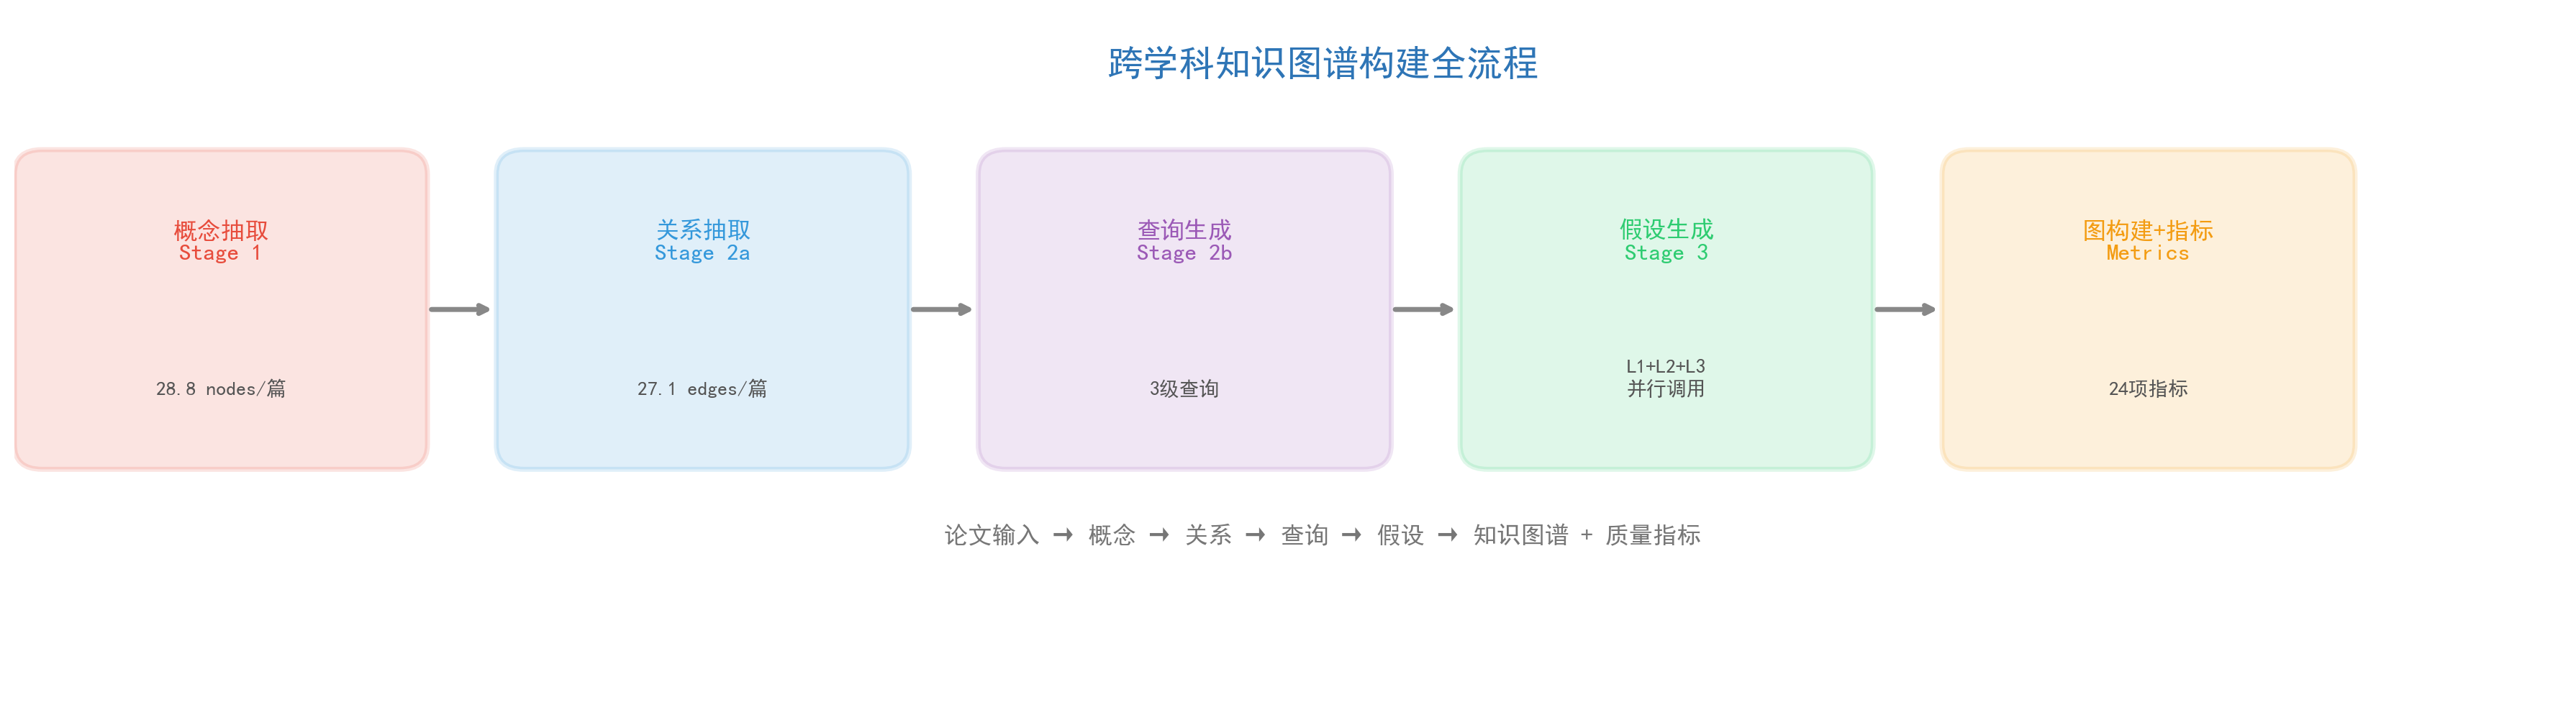
\includegraphics[width=\linewidth]{charts/pipeline_flow.png}
%     \caption{Overview of the multi-stage knowledge graph construction pipeline.}
%     \label{fig:pipeline}
% \end{figure}
%
% \begin{figure}[t]
%     \centering
%     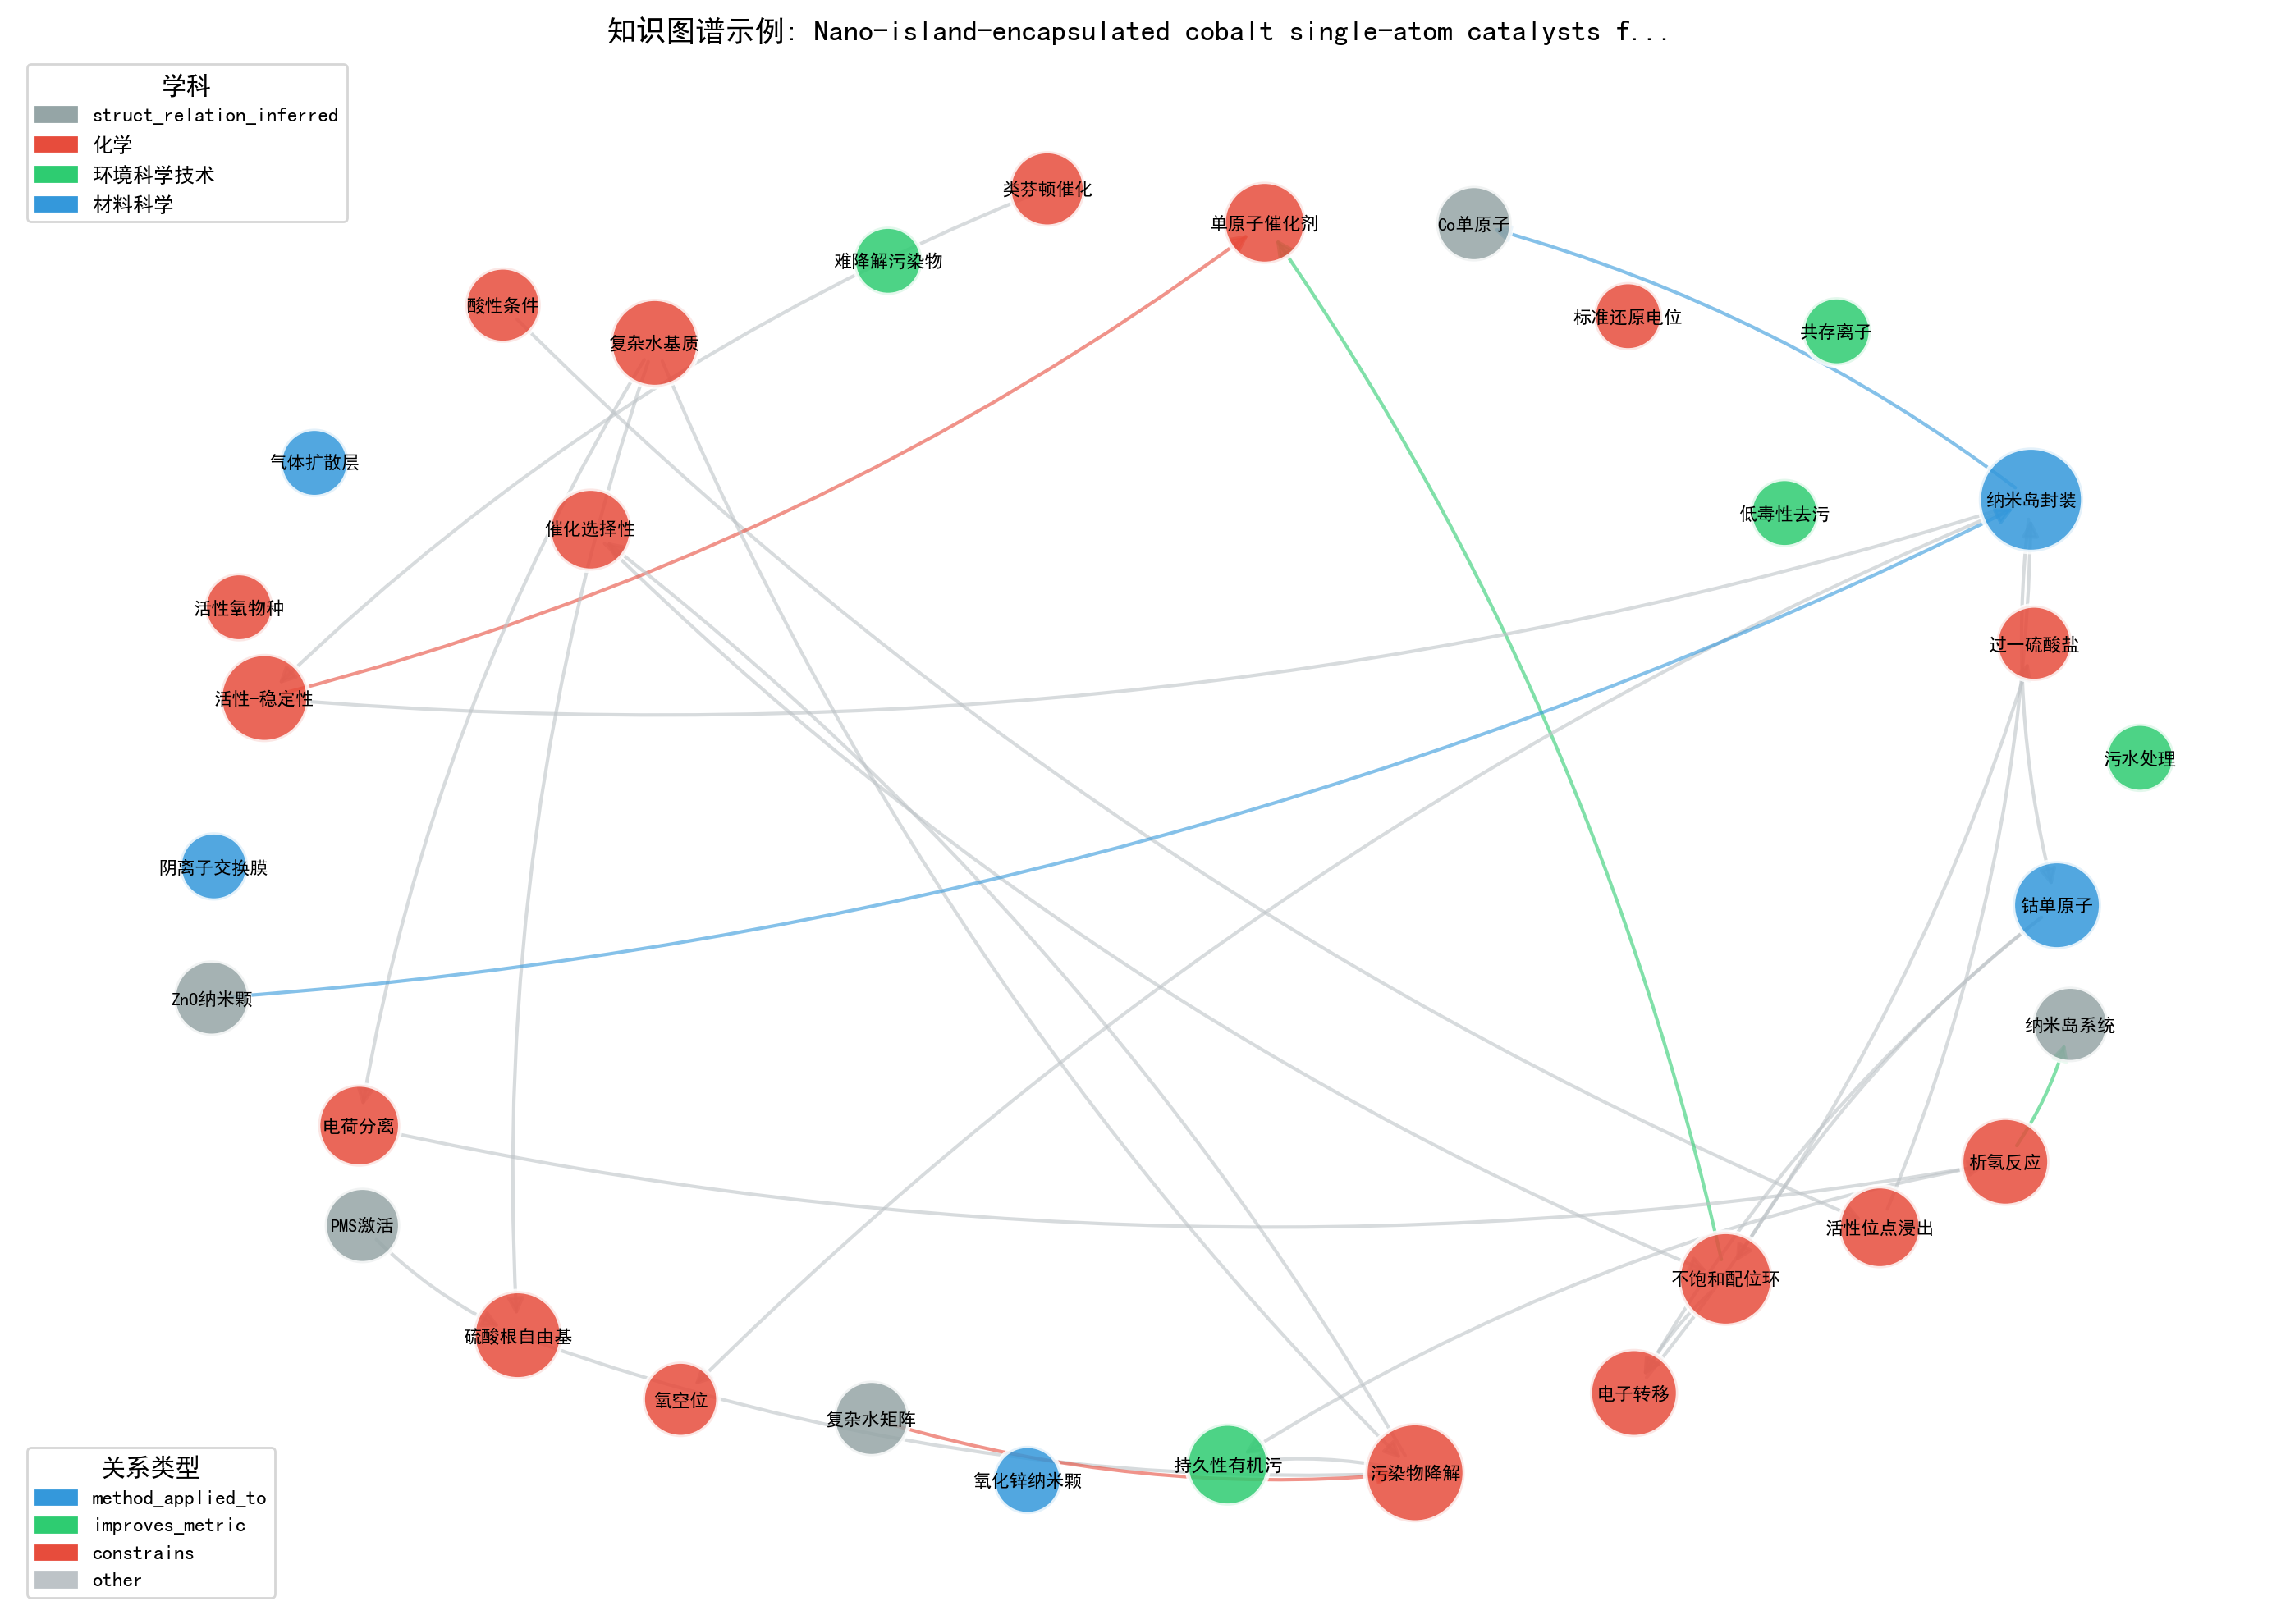
\includegraphics[width=0.9\linewidth]{charts/kg_example.png}
%     \caption{Example knowledge graph for a single paper. Nodes are colored by discipline; edges by relation type.}
%     \label{fig:kg_example}
% \end{figure}
%
% \begin{figure}[t]
%     \centering
%     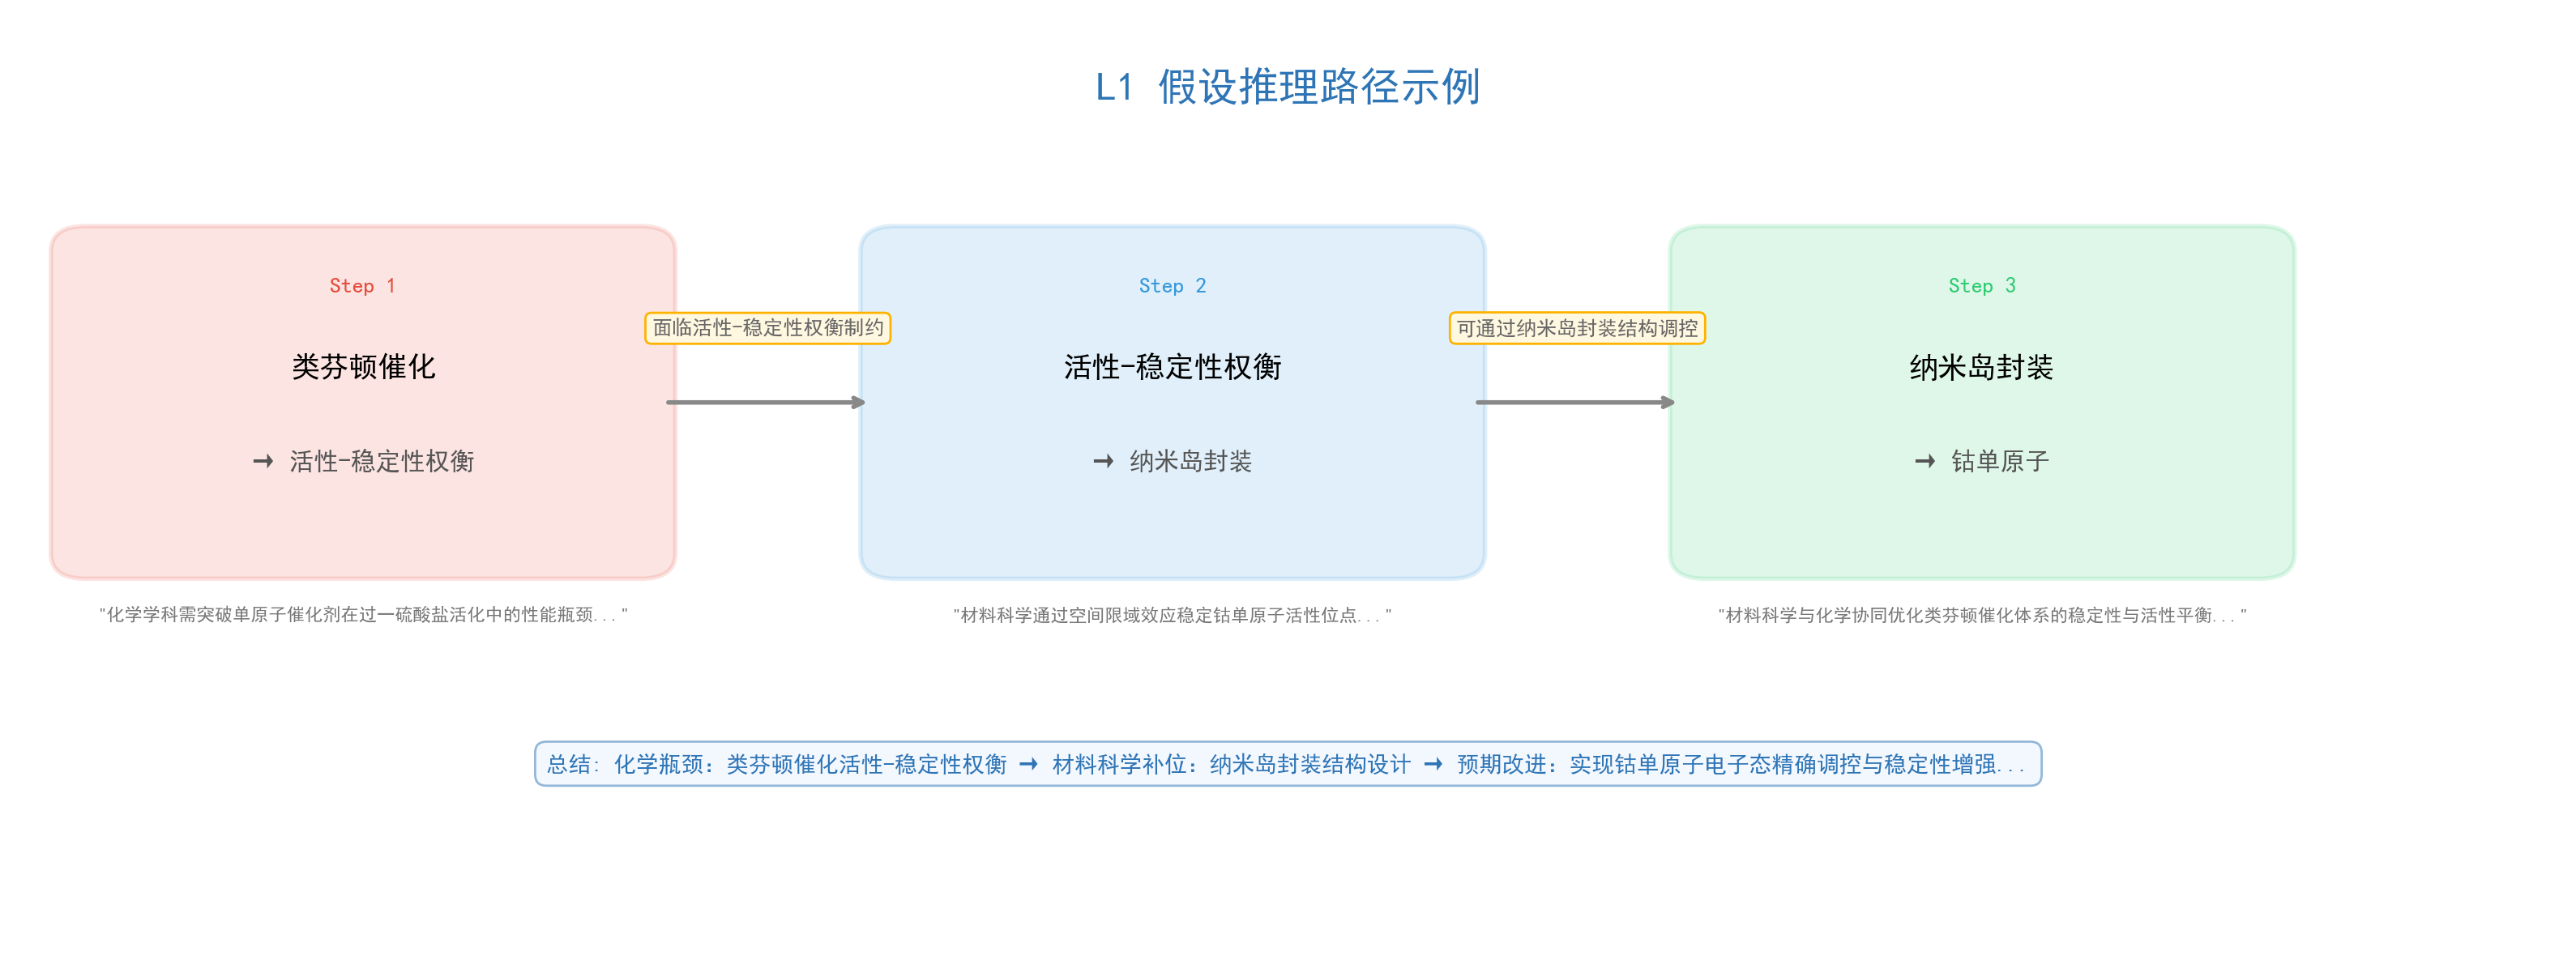
\includegraphics[width=\linewidth]{charts/hypothesis_chain.png}
%     \caption{Example L1 hypothesis reasoning path: a 3-step cross-disciplinary inference chain.}
%     \label{fig:hypothesis}
% \end{figure}
%
% \begin{figure}[t]
%     \centering
%     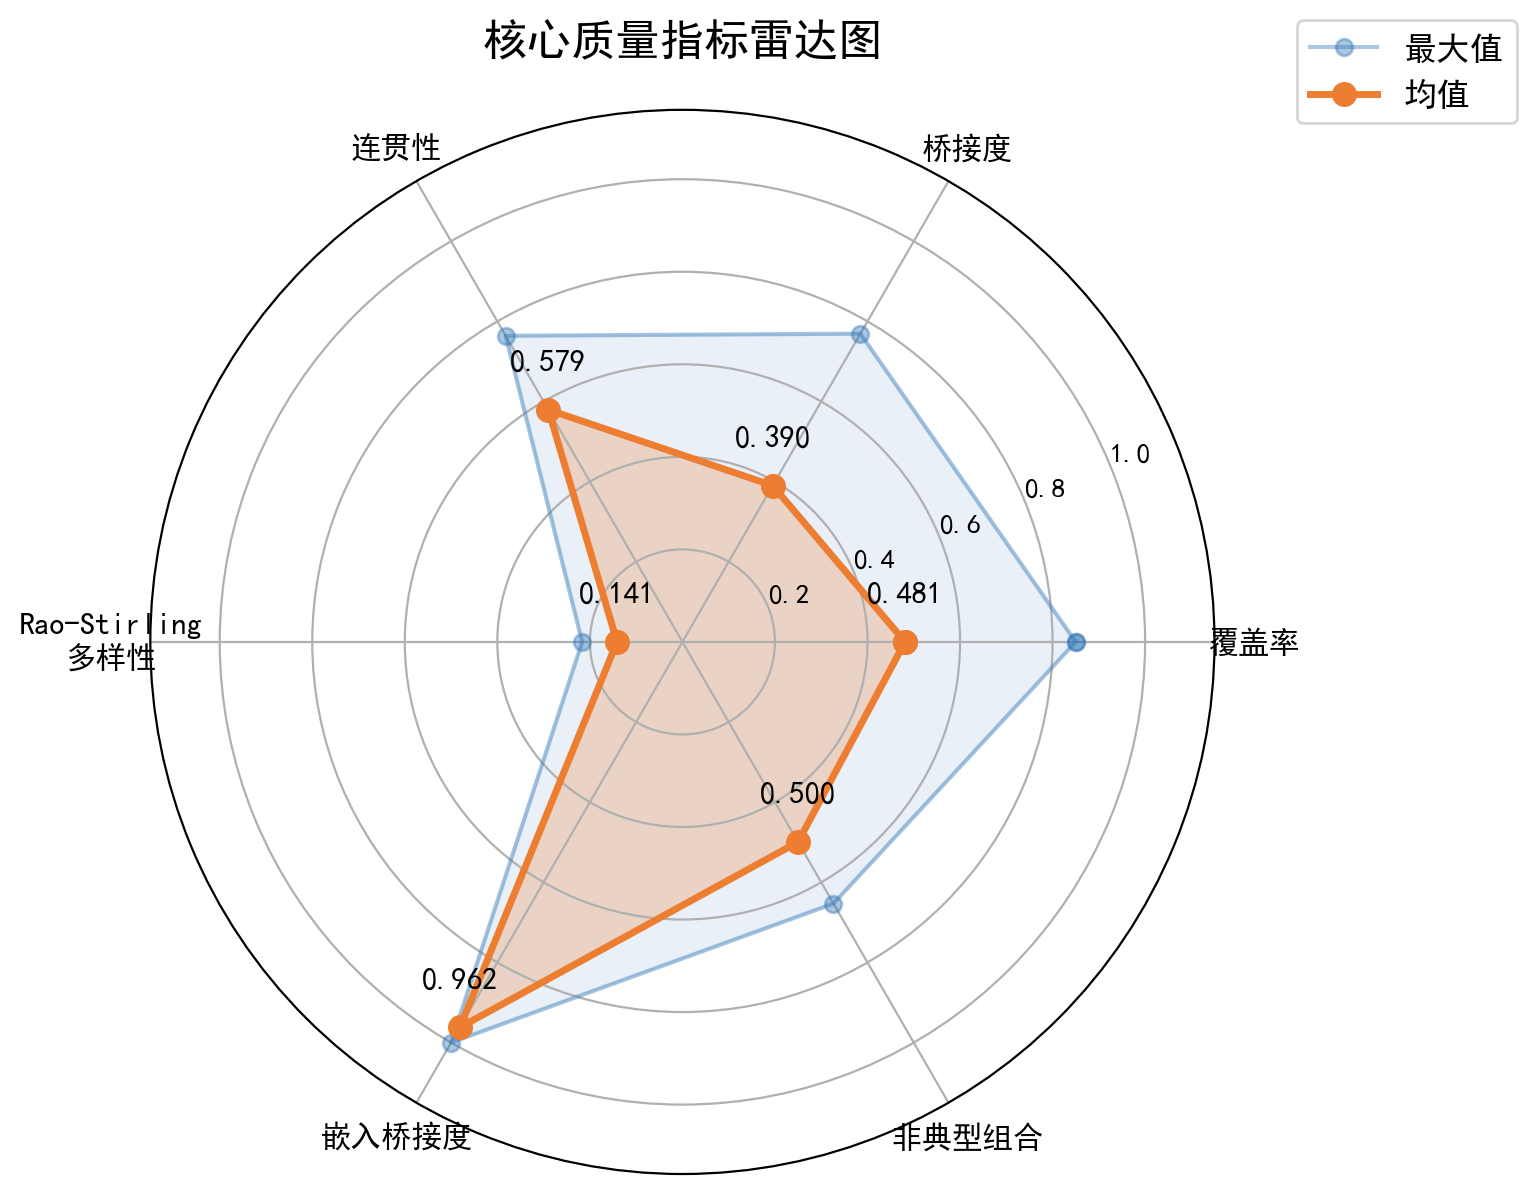
\includegraphics[width=0.8\linewidth]{charts/radar_metrics.png}
%     \caption{Radar chart of core quality metrics across 94 papers.}
%     \label{fig:radar}
% \end{figure}
%
% \begin{figure}[t]
%     \centering
%     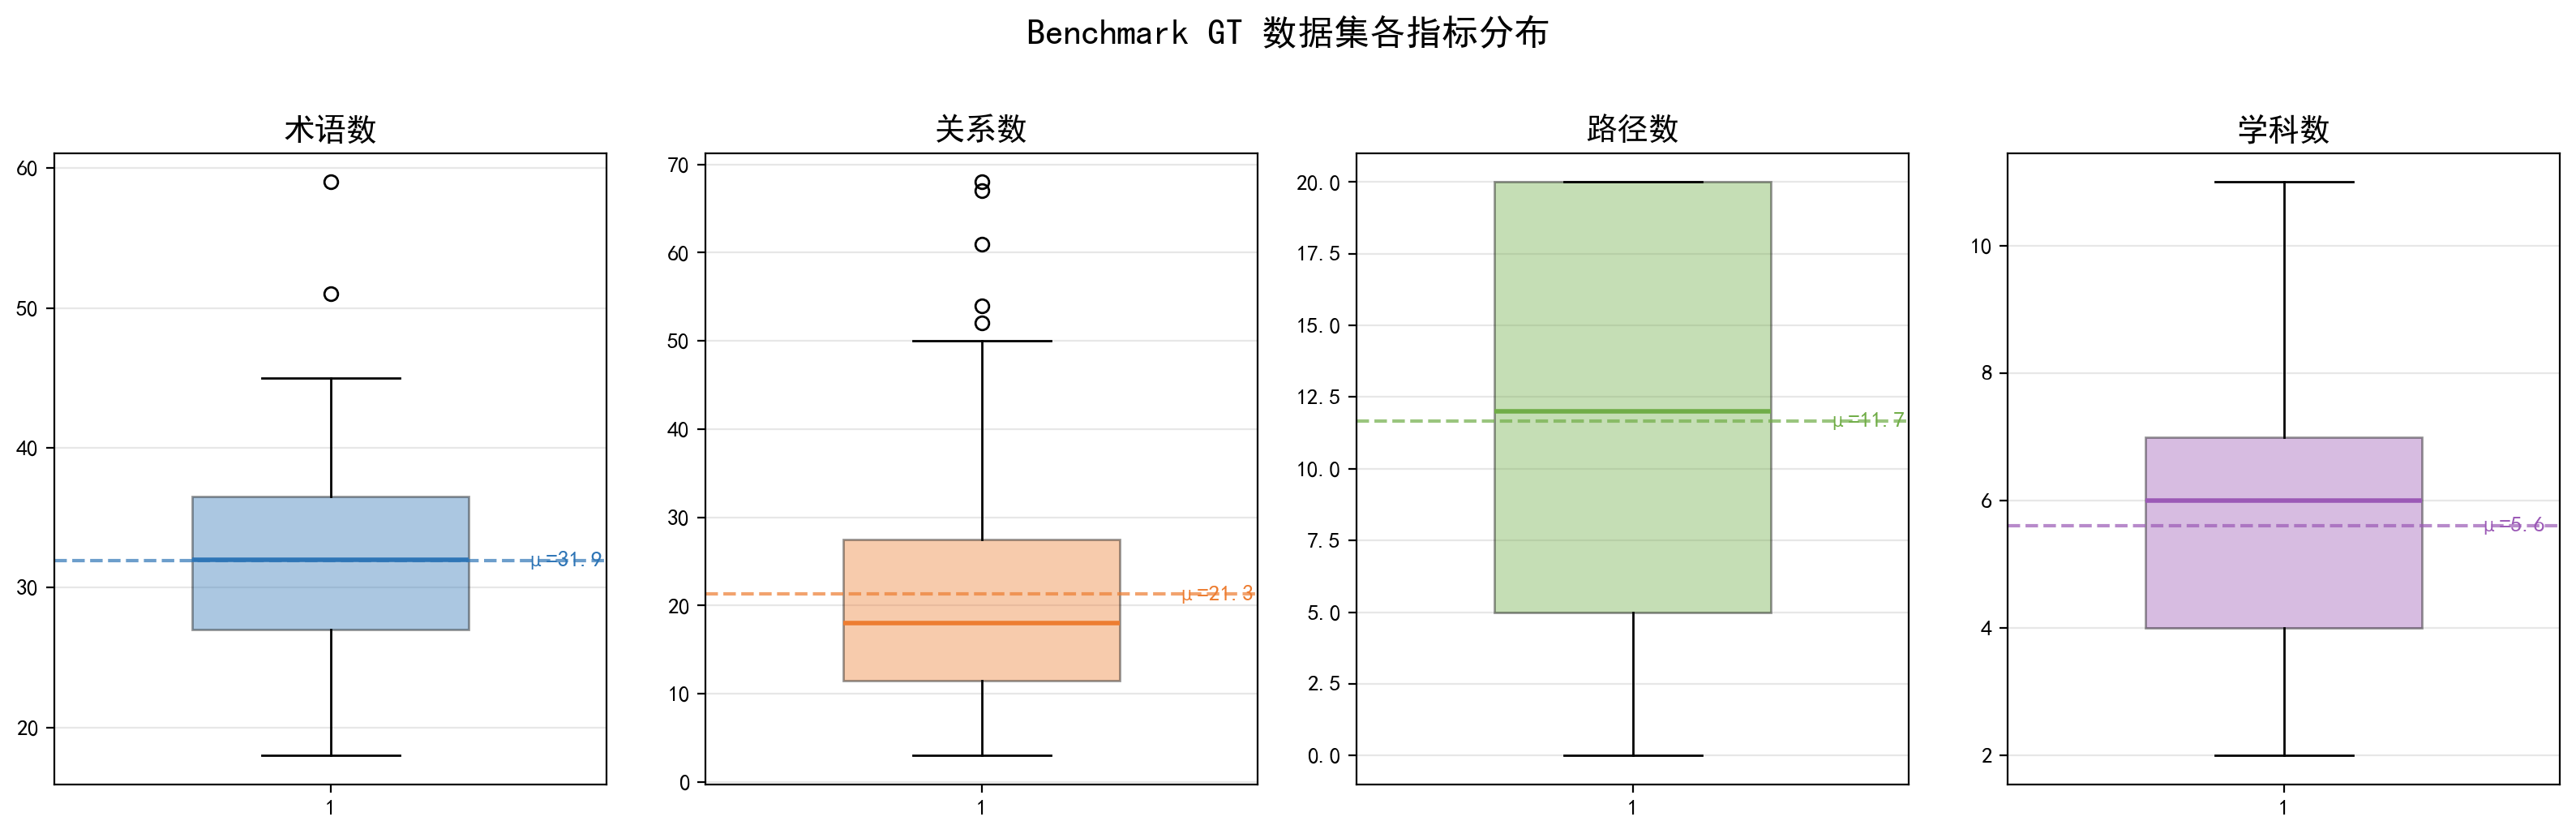
\includegraphics[width=\linewidth]{charts/benchmark_boxplot.png}
%     \caption{Distribution of benchmark GT dataset statistics.}
%     \label{fig:boxplot}
% \end{figure}
%
% \begin{figure}[t]
%     \centering
%     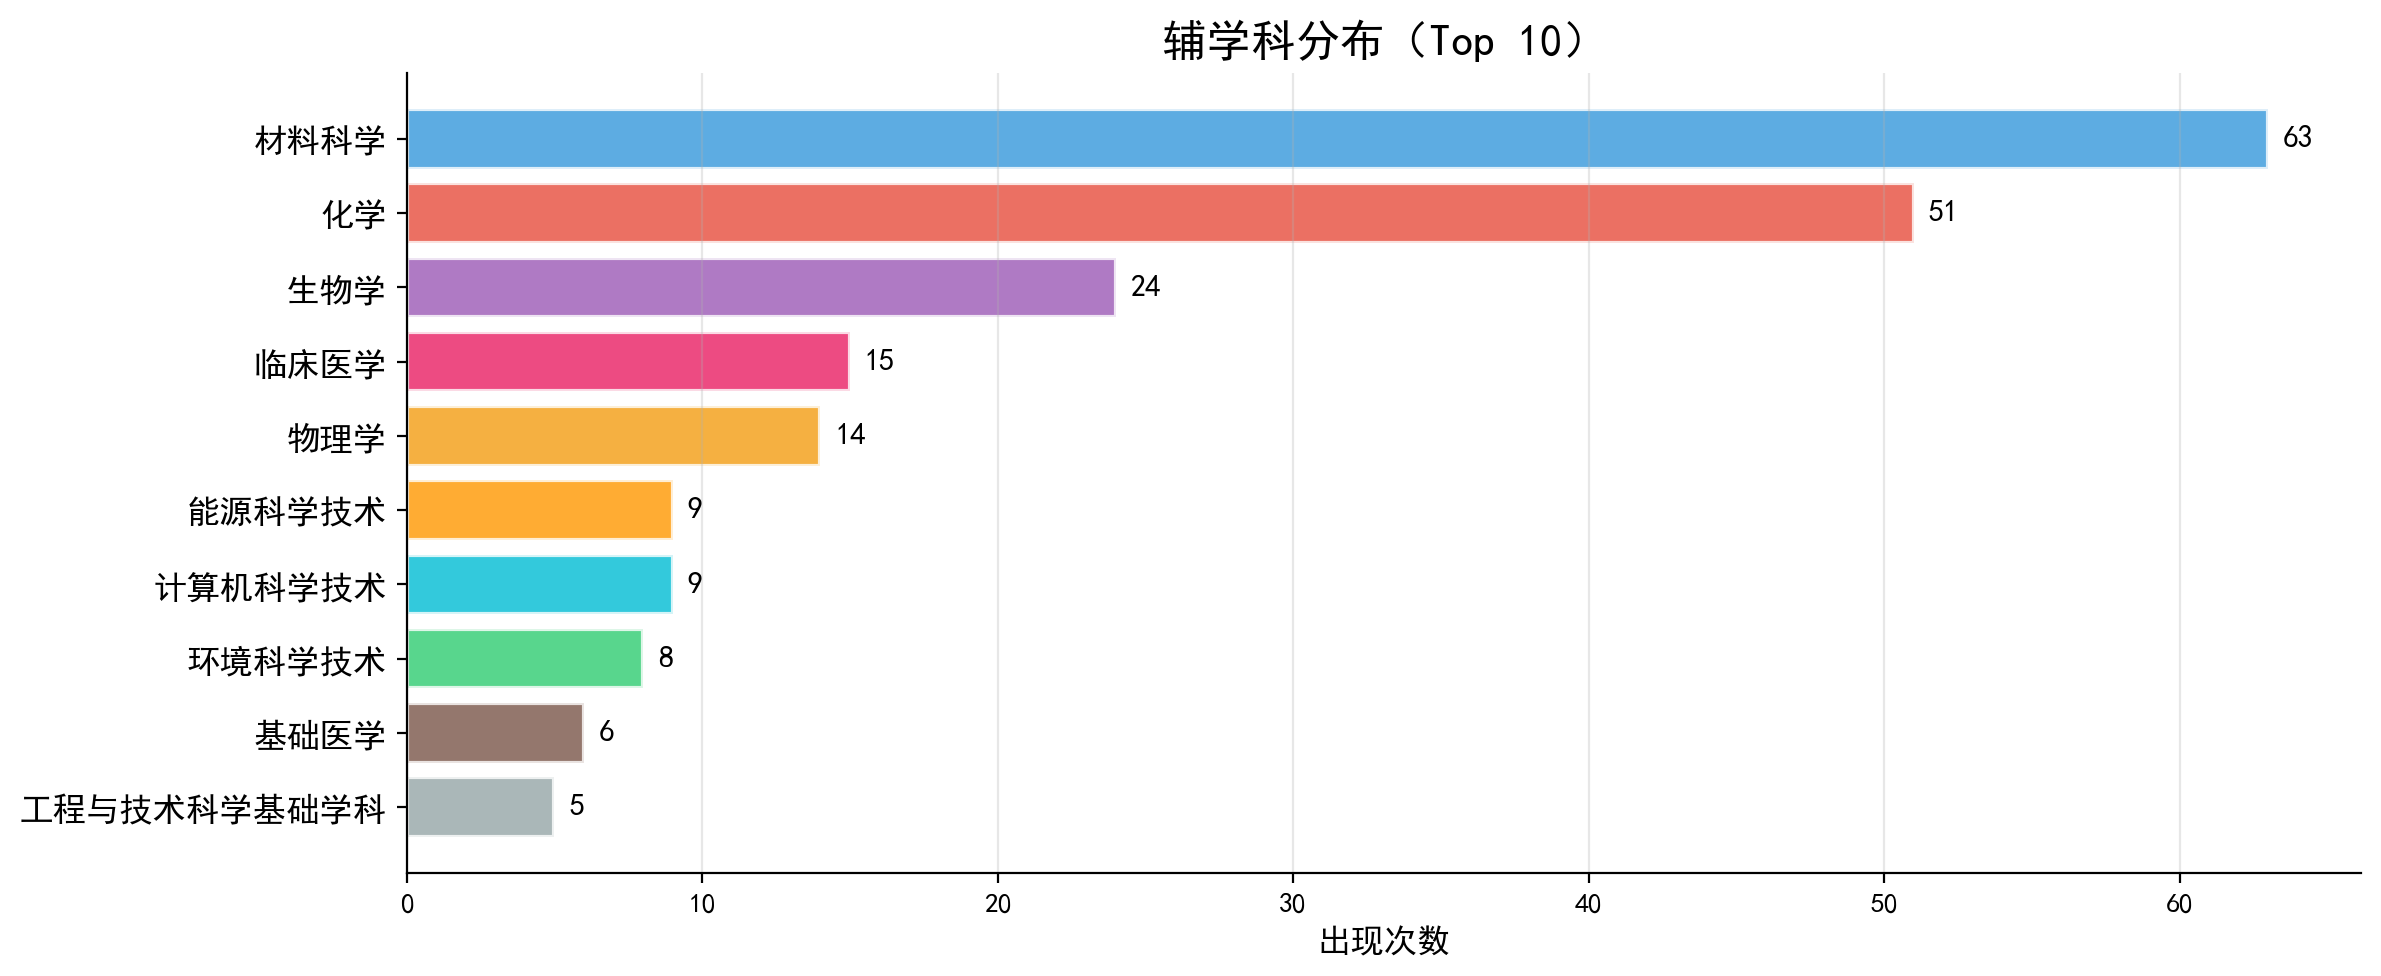
\includegraphics[width=0.9\linewidth]{charts/discipline_dist.png}
%     \caption{Top-10 secondary discipline distribution across 94 papers.}
%     \label{fig:discipline}
% \end{figure}
